\documentclass[paper=a4,fontsize=paper,12.5pt]{book}

\usepackage[margin = 1in,includefoot]{geometry} 
\usepackage{amsmath}
\usepackage{amssymb}
\usepackage{stix}
\usepackage{amsthm}
\usepackage{graphicx}
 \usepackage{tikz}
 \usepackage{polynom}
 \usepackage{hyperref}
 \usepackage{quiver}

\usepackage{mathtools}

\graphicspath{ {./meth_pic/} }
\usepackage{hyperref}

\newcommand{\3}{\vspace*{3mm}}
\newcommand{\Proof}{\textit{Proof:}}
\newcommand{\IFF}{$\Longleftrightarrow$ \hspace*{.5mm}}
\newcommand{\RIGHT}{\Longrightarrow \hspace*{.5mm}}
\newcommand{\LEFT}{\Longleftarrow \hspace*{.5mm}}
\newcommand{\coker}{\textnormal{coker} \hspace*{.5mm}}
\newcommand{\im }{\textnormal{im} \hspace*{.5mm}}
\newcommand{\Spec}{\textnormal{Spec}}
\newcommand{\cl}{\textnormal{cl}}
\newcommand{\Solution}{\textnormal{Solution}}
\newcommand{\tn}[1]{\textnormal{#1}}
\newcommand{\Fund}[2]{{\pi}_{1}(#1,#2)}
\newcommand{\fund}[1]{{\pi}_{1}(#1)}
\newcommand{\A}{\fund{\C{1}}}

\newcommand*{\comb}[2]{\binom{#1}{#2}}
\newcommand{\Z}{\mathbb{Z}}
\newcommand{\R}{\mathbb{R}}
\newcommand{\C}[1]{{S}^{#1}}
\newcommand{\FIG}[2]{
 \begin{figure}[!hbt]
 \begin{center}
 \begin{minipage}{0.85\textwidth}
 \centering{\includegraphics[width=90mm]{#1}}
 \caption{\label{#1}\small{#2}}
 \end{minipage}
 \end{center}
 \end{figure}
 }


\begin{document}

\newtheorem{lemma}{Lemma}
\newtheorem{sublemma}{Lemma}[lemma]
\newtheorem{theorem}{Theorem}
\newtheorem{conjecture}{Conjecture}

\newtheorem{definition}{Definition}[section]
\newtheorem{problem}{Problem}
\newtheorem{corollary}{Corollary}




\begin{theorem}

${\pi}_{1}({{S}^{1}}) \cong \Z$


\end{theorem}

\newpage

In layman terms this theorem basically says that every loop on the circle \textit{basically} has $3$ forms. Either we are looking at the loop which is constant, i.e stays on one point. The loop goes clockwise around the circle some amount of time, until ending where it started. Or the loop goes counter-clockwise some amount of times, until ending where it started.

\3

Now while that may be a self-evident fact, in the framework of algebraic topology it is very non-trivial and to prove it we must rely on the fact that the real line, $\R$ is a covering space of the circle $\C{1}$

\3

\begin{definition}

A space $C$ is the covering space of a space $X$ \IFF there exists a continuous map $p:C \to X$ such that for every $x \in X$ there is an open neighborhood of it, $U$, such that the pre-image ${p}^{-1}(U)$ is the disjoint union of open sets of $C$ such that each of them are homomorphically mapped onto $U$ by $p$


\end{definition}

\3

Now before we get to that we still need to define the homotopy group and even before that I must define what I mean by a path homotopy and more generally homotopy

\3

Also during this entire section when I use the term "map" I am referring to continuous functions, since the study of topology also includes the study of continuous functions which are the "special" maps of topological spaces. Formally, they are the arrows used in the definition of the category $\mathbf{Top}$.

\3

\begin{definition}

Given $2$ maps between $2$ spaces $X,Y$ a set of maps $\{{f}_{t}\}_{t \in I}$, where $I = [0,1]$ are a homotopy between $f$ and $g$ \IFF $H: I \times X \to Y$ defined by $H(t,x) = {f}_{t}(x)$ is continuous and $H(0,x) = f(x),H(1,x) = g$



\end{definition}

\3

While the definition may seem tricky the next definition about path homotopy is much more intuitive

\3

\begin{definition}

Given $2$ paths in the space $X$, i.e $f,g: I \to X$ which have the same endpoints, $f(0) = g(0), f(1) = g(1)$ a path homotopy is a homotopy such that the endpoints of each function in the homotopy are the same. 

\3

So if we had $H$ as defined before a path homotopy requires that $H(t,0)$ \&\ $H(t,1)$ are constant for all inputs $t$


\end{definition}

\3

Now to get an intuitive of this look at the following image and consider the paths ${f}_{0}$ and ${f}_{1}$. The paths in between the functions are to visualize the path homotopy between them, and what a path homotopy let's us do is basically consider the $2$ maps "equivalent" since one can be deformed into the other.

\3

{
 \begin{figure}[!hbt]
 \begin{center}
 \begin{minipage}{0.85\textwidth}
 \centering{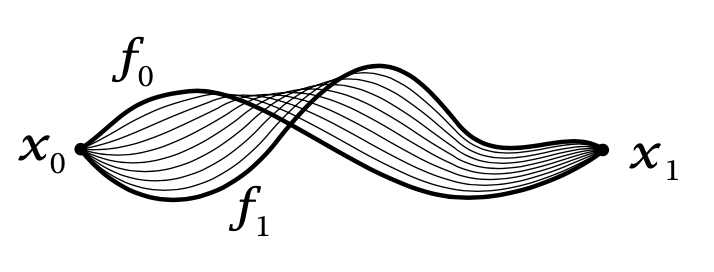
\includegraphics[width=45mm]{1}}
 \caption{\label{1}\small{Stolen from a book}}
 \end{minipage}
 \end{center}
 \end{figure}
 }

\3

Now why is this useful? Well because in other areas of "geometry" which is quite a loaded term, to classify certain objects it is REALLY important to know how many "holes" it has. I use quotes since holes in arbitrary spaces may not have a useful visualization. And different dimensional holes are quite odd, since we live in a $3$ dimensional world. But despite that in the study of $2$ dimensional surfaces the amount of holes, or "genus" of an object is crucial in studying it so ways to mimic the genus have been created. Mathematicians have done this through the concept of homotopy! 


\newpage

The intuition is that if we look at loops, paths who's endpoints are the same, on a space $X$ and considering 2 maps to be "the same" if they are path homotopic we can encounter holes. Consider a simple object such as the torus and notice the giant gaping hole it has in the middle of it. The way we can "encounter" it is by looking at loops which have to go through it. So any loop which has to go through the hole it has, can't be homotopic or be continuously deformed into a loop which never goes around the hole, since that would require us to split apart the loop if we would want to continuously deform it into the second loop.
\3


{
 \begin{figure}[!hbt]
 \begin{center}
 \begin{minipage}{0.85\textwidth}
 \centering{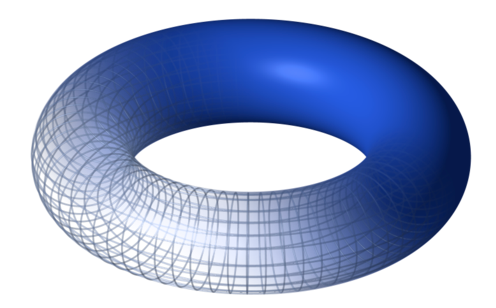
\includegraphics[width=45mm]{torus}}
 \caption{\label{torus}\small{Stolen from wikipedia}}
 \end{minipage}
 \end{center}
 \end{figure}
 }

\3

Okay so we got the intuition down but how exactly do we formally construct an algebraic object based on the concept of path homotopy. Well first of all we need to show that the relation "is path homotopic to" or usually notated "$\simeq$" holds the same properties as the usual equality relation $=$. This is so when we want to create an algebraic object, or specifically a group we can formally define the elements of said group, and have them be well behaved.

\3

\begin{lemma}

$\simeq$ is an equivalence relation




\end{lemma}

\Proof


Given any path $f$ in any space $X$ it is trivally path homotopic to itself by considering the constant homotopy ${f}_{t} = f$. If $f \simeq g$ and $H(t,x)$ is our path homotopy then we can consider the homotopy $H(1-t,x)$ from $g$ to $f$. This is trivally also a path homotopy between $g$ \&\ $f$.

\3

Finally if $f \simeq g$ and $g \simeq z$ then we have $2$ path homotopies $H$ and $H'$. We can define a third homotopy between $f$ and $z$ as $H''(t,x) = {f}_{2t}(x) $ for $0 \leq t \leq \frac{1}{2}$ and for $\frac{1}{2} \leq t \leq 1$ $H(t,x) = {g}_{2t - 1}$. Which informally means that for each map in the homotopy you go through $f$ twice as fast then go through $g$ twice as fast. Obviously we have that $H''(0,x) = H(0,x)$ and $H''(1,x) = H'(1,x)$. To prove continuity we use the fact that a function is continuous \IFF It is continuous when each time it is restricted to a finite amount of closed sets who's union is the domain. The closed sets which when restricted too $H''$ is obviously continuous are $[0,\frac{1}{2}] \times I$, $[\frac{1}{2} \times I]$, and $\{\frac{1}{2}\} \times I$. And since they are the entirety of $I \times I$ we are done $\QED$

\3

Now since $\simeq$ is an equivalence relation we can now consider the set ${\pi}_{1}(X,{x})$ of loops \textit{based at} $x$. The reason we have to identify some point of $X$ is because all of our loops have to start somewhere. Now while this is terrible for most topological spaces, for path-connected ones i.e for every $2$ points there is a path between them, the base point is irrelevant. I will prove this fact rigorously later.

\3

Now to make ${\pi}_{1}(X,{x})$ worth this amount of build-up we must define an operation on its elements. Which I will denote "$\cdot$" and is defined in the following way.

\3

Given any $2$ loops based at $x$ $f \cdot g$ is defined to be the loop $z$ which in the interval $t \in [0,\frac{1}{2}]$ is just $f(2t)$, and in the interval $[\frac{1}{2},1]$ is defined to be $g(2t-1)$. So given $2$ loops this operation $\cdot$ creates a loop which traces through the first loop at double speed, comes back to based point, then goes through the other loop at double speed and then stops at the base point.

\3

Now this operation is highly unstable in the set ${\pi}_{1}(X,{x})$ we tweak the definition of ${\pi}_{1}(X,{x})$ and define it to be the set of loops at base point $x$, modulo the path homotopy relation. We define the operation between equivalency classes the same may and instead taking the equivalence class of the new path created

\3

This still is a well defined definition of our operation due to the following lemma

\3

\begin{lemma}

If ${f}_{0} \simeq {f}_{1}$ and ${g}_{0} \simeq {g}_{1}$ $\RIGHT$ ${f}_{0} \cdot {f}_{1} \simeq {g}_{0} \cdot {g}_{1}$


\end{lemma}

\Proof

Since ${f}_{0} \simeq {f}_{1}$ and ${g}_{0} \simeq {g}_{1}$ we have path homotopies ${f}_{t}$ and ${g}_{t}$. We can then define a new path homotopy by $H(t,x) = ({f}_{t}(x) \cdot {g}_{t})(x)$. It is constant on the endpoints since $H(t,0) = ({f}_{t} \cdot {g}_{t})(0) = {f}_{t}(0)$ and $H(1,t) = ({f}_{t} \cdot {g}_{t})(1) = {g}_{t}(1)$. 

\3

The reason the map $H$ is continuous is because it is continuous on $[0,\frac{1}{2}] \times I$, and $[\frac{1}{2},1] \times I$ $\QED$

\3

We can now consider $\Fund{X}{x}$ as an algebraic object by endowing it with the operation $\cdot$. The following lemma shows that $\Fund{X}{x}$ is indeed a group.

\3

\begin{lemma}

 $\Fund{X}{x}$ is a group with operation $\cdot$ and identity $[c(s)]$ where $c(s) = 1$ for all $s \in [0,1]$


\end{lemma}

\Proof

Before we dive into the proof let me define what a reparametrization of a loop $f$. It is the composite map defined as $f\chi$ where $\chi: I \to I$ such that $\chi(0) = 0$ and $\chi(1) =1$. We have that $f\chi \simeq f$ by the path homotopy $f{\chi}_{t}$, ${\chi}_{t}(s) = (1-t)\chi(s) + ts$

\3

Now we can see trivially that $(f \cdot g) \cdot h \simeq f \cdot (g \cdot h)$ since they are just reparametrizations of each other since they traverse the same path but just as different speeds. 

\3

Let $f$ be some loop and let $c(s) = f(1)$. Then $f \cdot c \simeq f$ since $f\cdot c$ is the map which goes through $f$ twice as fast and stays on the endpoint in the interval $[\frac{1}{2},1]$. Thus $f \cdot c = f\chi$ where $\chi(s) = 2s$ for $0 \leq s \leq \frac{1}{2}$ and is just $f(1)$ on $[\frac{1}{2},1]$. Similarly $c \cdot f = f\psi$ where $\psi(s) = f(0) = f(1)$ on $[0,\frac{1}{2}]$ and on $[\frac{1}{2},1]$ is $2s$.

\3

Now given any path $f$ let $\bar{f}$ denote the inverse path $f(1-t)$ which starts at the endpoint of $f$, traces through $f$ and then ends at the startpoint of $f$. Given a loop $f$ consider the homotopy, ${f}_{t} \cdot {g}_{t}$ from $c(s) = f(0)$ to $f \cdot \bar{f}$. Where ${f}_{t}$ is $f$ on $[0,t]$ and $[t,1]$ is just equal to $f(t)$. And $g(t)$ is just the inverse path of ${f}_{t}$. Then this is a valid path homotopy since $({f}_{t} \cdot {g}_{t})(0)$ is always just $f(0)$ and $({f}_{t} \cdot {g}_{t})(1)$ is also just $f(0)$. Also the map $H(t,x) = ({f}_{t} \cdot {g}_{t})(x)$ is continuous trivially. So we have that $f \cdot \bar{f} \simeq c(s)$ and analgously we have that $\bar{f} \cdot f \simeq c(s)$ $\QED$

\3

Okay so now we know that $\Fund{X,x}$ is a valid group, but remember that I said that if we require a space to be path-connected, i.e any $2$ points have a path which connects them, we don't have to worry about our base point. Well now I can rigorously formulate this property

\3

\begin{lemma}

Let $h$ be a path from $x$ to $y$ then ${b}_{h}: \Fund{X,x} \to \Fund{X,y}$ is ${b}_{h}([f]) = [h \cdot f \cdot \bar{h}]$ is an isomorphism 


\end{lemma}

\Proof

It is well defined since if ${f}_{t}$ is a homotopy from a loop $f$ to $g$ then $h \cdot {f}_{t} \cdot \bar{h}$ is a homotopy from $h \cdot f \cdot \bar{h}$ and $h \cdot g \cdot \bar{h}$

\3

It is a homomorphism since ${b}_{h}[f \cdot g] = [h \cdot f \cdot g \cdot \bar{h}] = [ h \cdot f \cdot \bar{h} \cdot h \cdot g \cdot \bar{h}] = {b}_{h}[f]{b}_{h}[g]$

\3

It is bijective and its functional inverse is ${b}_{\bar{h}}$ since ${b}_{h}({b}_{\bar{h}}[f]) = {b}_{h}[\bar{h} \cdot f \cdot h] = [f]$ and similarly ${b}_{\bar{h}}({b}_{h}[f]) = {b}_{\bar{h}}[h \cdot f \cdot \bar{h}] = [f]$ $\QED$


\newpage


Now we can actually get to proving that $\fund{\C{1}} \cong \Z$

\3

The main part of the proof is the map $p: \R \to \C{1}$ defined by the rule $p(s) = (\cos 2\pi s, \sin 2\pi s)$

\3

One can imagine this map as the composition of $2$ maps. The first map being the embedding of $\R$ into ${\mathbb{R}}^{3}$ as a helix via $f(x) = (\cos 2\pi s, \sin 2\pi s,s)$ and secondly a projection of this helix onto $\C{1}$ by just removing the $z$-coordinate. Here's an image showing the map from the the helix to the circle. 

\3

{
 \begin{figure}[!hbt]
 \begin{center}
 \begin{minipage}{0.85\textwidth}
 \centering{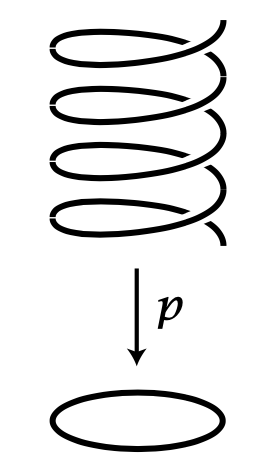
\includegraphics[width=25mm]{helix}}
 \caption{\label{helix}\small{Stolen from Hatcher}}
 \end{minipage}
 \end{center}
 \end{figure}
 }

\3

Now one can somewhat see the intuition behind the definition of a covering space which I gave at the start of this section, but I will just put it here again. Every pre-image of a neighborhood of a point on the circle maps to countably many neighborhoods on the helix

\3

\begin{definition}

A space $C$ is the covering space of a space $X$ \IFF there exists a continuous map $p:C \to X$ such that for every $x \in X$ there is an open neighborhood of it, $U$, such that the pre-image ${p}^{-1}(U)$ is the disjoint union of open sets of $C$ such that each of them are homomorphically mapped onto $U$ by $p$


\end{definition}

\3

Now finally I can start with the first definition on our journey of proving that the fundamental group, ${\pi}_{1}(X)$ of the circle is $\Z$. 

\3

Also the reason I don't specify a base point is because $\C{1}$ is path-connected

\3

\begin{definition}

$\psi: \Z \to \A$ is defined as $\psi(n) = [{w}_{n}(s)]$ where ${w}_{n}(s) = (\cos 2\pi ns, \sin 2\pi ns)$

\3

Notice that ${w}_{n}(s) = (p \circ {f}_{n})(s)$ where ${f}_{n}(s) = ns$ which is a path from $0$ to $n$

\end{definition}

\3

\begin{lemma}

$\psi(n) = [pf]$ where $f$ is any path from $0$ to $n$


\end{lemma}

\Proof

Trivial since we already have that $p{f}_{n} = {w}_{n}(s)$ and since any $2$ paths in $\R$ are path homotopic the lemma is true $\QED$

\3

\begin{lemma}

$\psi$ is a homorphism


\end{lemma} 


\Proof

Let ${t}_{m}$ denote the translation ${t}_{m}(x) = x + m$. Then we have that $\psi(m+n) = [p({f}_{m} \cdot ( {t}_{m} \circ {f}_{n}))]$ due to lemma $6$. But $p({f}_{m} \cdot ( {t}_{m} \circ {f}_{n})) = {w}_{m} \cdot {w}_{n}$ and thus $\psi(m+n) = \psi(m) \cdot \psi(n)$ $\QED$


\newpage

Now we just need to show that $\psi$ is bijective. We do this by first introducing the concept of a lift. Given any path $f$ in $\C{1}$ a lift is a path in $\R$, $f'$ such that $pf' = f$.

\3

Now I can state $2$ statements which prove that $\psi$ is bijective

\begin{enumerate}

\item Given any path $f$ in $\C{1}$ that starts at $x$ then for any $y \in {p}^{-1}(x)$ there is a unique lift $f'$ of $f$ which starts at $y$

\item Given any path homotopy ${f}_{t}$ starting at $x$ then for any $y \in {p}^{-1}(x)$ there is a unique homotopy of lifts of each of the ${f}_{t}$, ${f'}_{t}$ which start at $y$

\end{enumerate}

\3

Now let's show that these imply that $\psi$ is bijective

\3

To show that $\psi$ is surjective let us first fix $(1,0)$ as the base point we are working with. And let $f$ be a path starting at $(1,0)$ then there is unique lift by $(1)$ $f'$ which is a path from $0$ to some integer $n$ since $f'(1)$ must be such that $pf'(1) = f(1) = (1,0)$ and we have that $ {p}^{-1}(1,0) = \Z$. So by lemma $6$ $\psi(n) = [f]$

\3

To show that $\psi$ is injective let $n$ and $m$ be such that ${w}_{n} \simeq {w}_{m}$. Then by $(2)$ there is unique lifted path homotopy from ${f}_{n}$ to ${f}_{m}$ which starts from $0$. Since this is a path homotopy the end points must be constant for any map in the homotopy, which I will denote as ${f}_{t}$. So ${f}_{1}(1) = {f}_{m}(1) = m$ and since ${f}_{0}(1) = {w}_{n}(1) = n$ we have that $n = m$.

\3

Now we just need to prove those $2$ statements but due to the following lemma we just need to prove one general statement


\begin{lemma}

If given any map $F: Y \times I \to \C{1}$ and a map $F': Y \times \{0\} \to \R$ which lifts $F$ restricted to $Y \times \{0\}$ then there is a unique extension of $F'$, $F'': Y \times I \to \R$ such that  $pF' = F$ THEN the $2$ statements which I stated above are true
 

\end{lemma}

\Proof 

For the first statement given any path in $\C{1}$ by our hypothesis if $Y$ is just a point and we make $f$ our $F$, $f(0)$ represent $F$ and any point $y$ such that $p(y) = f(0)$ represent our $F'$ then we have a map $F'':I \to \R$, or rather a path in $\R$ which lifts $F$ or rather our original path $f$

\3

For the second statement if we have any homotopy of paths in $\C{1}$ denoted ${f}_{t}$, i.e a map $F: I \times I \to \C{1}$ then our $F'$ would just be a lift of $F:I \times \{0\} \to \C{1}$ or rather ${f}_{0}(x)$ which we knows should exist due to the above proof. Then by our hypothesis $F'$ can be uniquely extended to a map $F'': I \times I \to \R$. And when we restrict $F''$ to $I \times \{0\}$ and $I \times \{1\}$ we get lifts of the constant path at ${x} = {f}_{t}(0)$ and by uniqueness we have that $F''$ is a homotopy of paths $\QED$



Now we're almost done 
\newpage

\begin{theorem}

If given any map $F: Y \times I \to \C{1}$ and a map $F': Y \times \{0\} \to \R$ which lifts $F$ restricted to $Y \times \{0\}$ then there is a unique extension of $F'$, $F'': Y \times I \to \R$ such that  $pF' = F$

\end{theorem}

\Proof

Before I get to the meat of the proof let me just state what we already know. $F$ is a map from $Y \times I \to \C{1}$, $F'$ is a map from $Y \times \{0\} \to \R$ which is a lift of $F$ when it is restricted to $Y \times \{0\}$. 

\3

Now we construct $F''$ for any neighborhood of a point of $y$. So let $y \in Y$ and let $ y \in U$ be open. Since $F$ is continuous any point $(y,t) \in Y \times I$ has a neighborhood ${U}_{t} \times ({a}_{t},{b}_{t})$ such that $F({U}_{t} \times ({a}_{t},{b}_{t})) \subset {V}_{\alpha}$ for some evenly covered neighborhood of $F({y}_{0},{t}_{0})$. Which is a neighborhood such that there exist a disjoint collection of neighborhoods in $\R$ which are mapped homeomorphically onto said neighborhood or rather evenly covered

\3

Since $I \times \{y\}$ is compact there are finitely many ${V}_{t} \times ({a}_{t},{b}_{t})$ which cover $\{y\} \times I$. So given our neighborhood $U$ of $y$ we can choose ${t}_{i}$ such that $0 = {t}_{0} < ... < {t}_{n} = 1$ and such that $F(U \times [{t}_{i},{t}_{i+1}]) \subset {V}_{i}$ where ${V}_{i}$ is some evenly covered neighborhood. 

\3

Let's then proceed by induction. 

\3

We'll be doing induction of the following statement

\3

$F''$ is a well-defined map on $U \times [0,{t}_{i}]$ and lifts $F$  $\equiv P(i)$

\3

The statement $P(0)$ is already given since we can just define it as $F'$ when restricted to $U \times \{0\} \subset Y \times \{0\} $

\3

Then inductively that $F''$ is defined on $U \times [0,{t}_{i}]$. Then by our definition of covering space there should exist open sets of $\R$ such that ${V'}_{i}$ which are mapped homemorphically onto ${V}_{i}$ by $p$ which also contains the point $F''(y,{t}_{i})$ we also can assume that $F''( U \times \{{t}_{i} \}) \subset {V'}_{i}$ by replacing $U$ with a smaller neighborhood by say $U \bigcap {F'' |(U \times {{t}_{i}})}^{-1}({V'}_{i})$. Now we can define $F''$ on $U \times [{t}_{i}, {t}_{i+1}]$ by ${p}^{-1}F$ by considering ${p}^{-1}$ to be the homemorphism of ${V}_{i}$ onto ${V'}_{i}$. We then finally get $F''$ to be a fully defined map from $U \times I \to \R$

\3

Now we need to prove the uniqueness of $F''$ when $Y$ is a point
\3

Given any $2$ lifts, $z,g$, of a path on $\C{1}$, $f$ such that $z(0) = g(0)$ we can attempt to the thing we did before. Choose some partition of $[0,1]$, ${t}_{i}$ such that $F([{t}_{i},{t}_{i+1}]) \subset {V}_{i}$. 

\3

Assume inductively that $z =g$ on $[0,{t}_{i}]$.Since $[{t}_{i},{t}_{i+1}]$ is connected $z([{t}_{i},{t}_{i+1}])$ is connected and thus must lie in exactly $1$ ${V'}_{i}$. And thus the same is for $g$ since $z({t}_{i}) = g({t}_{i})$. And since $z$ and $g$ are lifts of $f$ even when restricted to $z[{t}_{i},{t}_{i+1}] $ and $g[{t}_{i},{t}_{i+1}]$ we have that $p(z) = p(g)$ when we restrict them to ${V'}_{i}$. Since $p$ is injective when restricted to ${V'}_{i}$ we have that $z = g$ 

\3

Now the final step is to show that in general we can lift $F''$ to a map defined on $Y \times I$. By the preceding proof for any open set $U$ we can construct $F''$ on $U \times I$. Whenever we have a $(y,t) \in U \bigcap U' \times I$ $F''(y,t)$ is uniquely determined since any lift of this manner on a single segment $\{y\} \times I$ is automatically unique, so constructing $F''$ globally via open sets will be unique on each intersection.

\3

Finally $F''$ is continuous on $Y \times I$ since it is continuous when restricted to any set of the form $U \times I$ where $U \subset \C{1}$ $\QED$

\newpage

Now FINALLY I can state the following

\begin{corollary}

${\pi}_{1}(\C{1}) \cong \Z$

\end{corollary} 

\3

This last section is just a nice application of what we just proved

\3

\begin{theorem}

Every non-constant polynomial with complex coefficients has a complex root


\end{theorem}

\Proof

For the sake of contradiction let $p$ be a non-constant polynomial that has no root. WLOG $p(z) = {z}^{n} + {a}_{n-1}{z}^{n-1} + ... {a}_{0}$

\3

Since $p(z)$ has no roots we can define ${f}_{r}(s) = \frac{p(r{e}^{2\pi i s})/p(r)}{|p(r{e}^{2\pi i s})/p(r)|}$ for any $r \geq 0$ and this defines a loop on the unit circle $\C{1}$ when it is considered to be a part of the complex plane. If $r = 0$ then we get the constant map and since as $r$ varies we have a path homotopy between all of the ${f}_{r}$ we have that $[f_{r}] = [{w}_{0}]$ where ${w}_{0}$ denotes the constant map for the start/end point of ${f}_{r}$.

\3

Now consider a real number $r$ such that it is larger than $1 + |{a}_{0}| + .. + |{a}_{n-1}|$ then we have the following inequalities if $|z| = r$

\3

\[|{z}^{n}| = {r}^{n} = {r}{r}^{n-1} > (|a_{0}| + .. + |a_{n-1}|){|z|}^{n-1} \geq |p(z) - {z}^{n}| \]

\3

The inequalities above imply that for $t \in I$ the polynomial $p_{t}(z) = {z}^{n} + t(p(z) - {z}^{n})$ must have no roots on the circle $|z| = r$.


Since if it did for some $|z| = r$ then we would have that $|{z}^{n}| = t|p(z) - {z}^{n}| \leq |p(z) - {z}^{n}|$ which would contradict our above inequality.

\3

Now let $r$ be as above and define ${F}_{t}(s) = \frac{p_{t}(r{e}^{2\pi i s})/p_{t}(r)}{|p_{t}(r{e}^{2\pi i s})/p_{t}(r)|}$. Now consider the homotopy from $t = 1$ to $t = 0$. It is a homotopy from ${F}_{1}$ which remember is still homotopic to the constant map. And $F_{0}(s) = \frac{p_{t}(r{e}^{2\pi i s})/p_{t}(r)}{|p_{t}(r{e}^{2\pi i s})/p_{t}(r)|} = \frac{e^{2 \pi i n s}}{|{e}^{2\pi i n s}|} $ which is equal to ${e}^{2\pi i n s} = {w}_{n}(s)$ and thus we have that ${w}_{n}(s) \simeq {w}_{0}(s)$ which implies that $n = 0$ $\QED$

\3










\end{document}